\section{Historique}

\begin{frame}{Retour sur les bases de données relationnelles}

    Les bases de données relationnelles permettent de stocker des \textbf{données structurées} dans des \textbf{relations} (également appelées tables).

    \begin{figure}[htb]
        \centering
        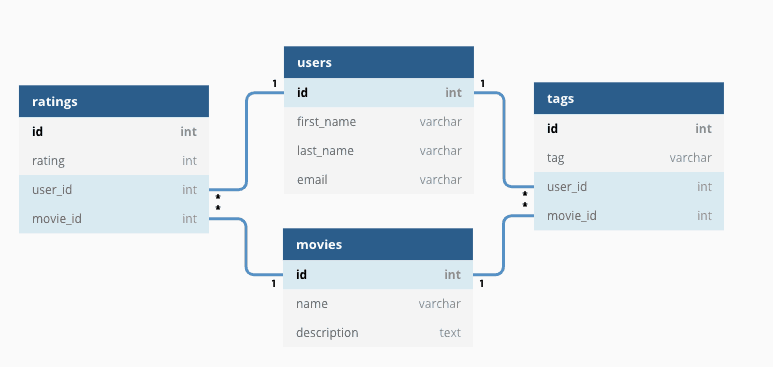
\includegraphics[width=0.8\textwidth]{img/relational-database.png}
    \end{figure}

\end{frame}

\begin{frame}{Modèle relationnel}
    \begin{tikzpicture}
    % Define classes
    \umlclass[x=0,y=0]{Customer}{
        - id : int \\
        - name : String \\
        - email : String
    }{
        + placeOrder() : void \\
        + cancelOrder() : void
    }

    \umlclass[x=5, y=0]{Order}{
        - orderId : int \\
        - date : Date
    }{
        + addProduct(Product) : void \\
        + calculateTotal() : float
    }

    \umlclass[x=5, y=-4]{Product}{
        - productId : int \\
        - name : String \\
        - price : float
    }{
        + applyDiscount(float) : void
    }

    % Relationships
    \umlassoc[arg1=1, pos1=0.2, arg2=*, pos2=0.8]{Customer}{Order}
    \umluniassoc[mult1=1, mult2=*, pos2=0.8]{Order}{Product}
    \umlcompo[mult1=1, mult2=1..*, pos2=0.8]{Customer}{Product}
\end{tikzpicture}
\end{frame}

\begin{frame}{Changement de paradigme}

    \begin{itemize}
        \item \textbf{Années 2000} : explosion du volume de données
        \item \textbf{Modèle relationnel} : limité en termes de \textbf{scalabilité} et de \textbf{flexibilité}
        \item \textbf{Nouvelles technologies} : Big Data, IoT, applications web et mobiles
    \end{itemize}

\end{frame}

\begin{frame}{Normalisation vs dénormalisation}

    \begin{itemize}
        \item \textbf{Modèle relationnel} : normalisation des données
        \item \textbf{Modèle NoSQL} : dénormalisation des données
    \end{itemize}

    Donner exemple

    Formes normales : 1NF, 2NF, 3NF, BCNF, 4NF, 5NF
\end{frame}

\begin{frame}{Formes normales}

    En informatique, une \textbf{forme normale} est un ensemble de règles visant à organiser les données dans une base de données relationnelle afin de minimiser la redondance et d'améliorer l'intégrité des données.
    % https://www.datacamp.com/tutorial/normalization-in-sql
    \begin{itemize}
        \item \textbf{1NF} : élimination des groupes de répétition
        \item \textbf{2NF} : élimination des dépendances partielles
        \item \textbf{3NF} : élimination des dépendances transitives
        \item \textbf{BCNF} : Boyce-Codd Normal Form
        \item \textbf{4NF} : élimination des dépendances multivaluées
        \item \textbf{5NF} : élimination des dépendances de jointure
%        \item \textbf{DNF} : forme dénormalisée
%        \item \textbf{ENF} : forme normalisée étendue
%        \item \textbf{ONF} : forme normale optimale
%        \item \textbf{TNF} : forme normale temporelle
%        \item \textbf{INF} : forme normale d'inclusion
%        \item \textbf{PNF} : forme normale de projection
%        \item \textbf{KNF} : forme normale de clé
%        \item \textbf{LNF} : forme normale logique
%        \item \textbf{MNF} : forme normale minimale
%        \item \textbf{NNF} : forme normale négative
    \end{itemize}

\end{frame}

\begin{frame}{Application de formes normales}

    Exemple de formes normales sur une table de base de données relationnelle.

\end{frame}

\begin{frame}{OLAP vs OLTP}

    \begin{itemize}
        \item \textbf{OLTP} : Online Transaction Processing
        \item \textbf{OLAP} : Online Analytical Processing
    \end{itemize}

    OLAP : requêtes complexes, agrégations, analyses multidimensionnelles

    OLTP : transactions, insertions, mises à jour, suppressions

\end{frame}
